\documentclass[final,5p,times,twocolumn]{elsarticle}

% ==============================================================================
% Packages & Environment Setup
% ==============================================================================
\usepackage{amsmath,amssymb,amsfonts,amsthm}
\usepackage{bm}
\usepackage{graphicx}
\graphicspath{{./}{../figures/}}
\usepackage{booktabs}
\usepackage{tabularx}
\usepackage{subcaption}
\usepackage{microtype}
\usepackage{algorithm}
\usepackage{algpseudocode}
\usepackage{tikz}
\usetikzlibrary{shapes.geometric, arrows, positioning, fit, calc}
\usepackage{hyperref}

\hypersetup{
    colorlinks=true,
    linkcolor=blue,
    citecolor=blue,
    urlcolor=blue,
    pdftitle={Parameterized Reduced Order Modeling in Structural Dynamics via Isogeometric Analysis},
    pdfauthor={Mumen Wehbe}
}

\journal{Computer Methods in Applied Mechanics and Engineering}

% ==============================================================================
% Document Body
% ==============================================================================
\begin{document}

\begin{frontmatter}

\title{Projection-based Reduced Order Modeling for Structural Dynamics via Isogeometric Analysis and Hyper-Reduction}

\author[1]{Mumen Wehbe\corref{cor1}}
\ead{mumen.wehbe@lecnam.net}
\cortext[cor1]{Corresponding author}

\address[1]{Conservatoire National des Arts et Métiers (Cnam), 292 Rue Saint-Martin, 75003 Paris, France}

% ------------------------------------------------------------------------------
% Abstract
% ------------------------------------------------------------------------------
\begin{abstract}
Real-time digital twins of complex elastodynamic structures require both geometrically exact discretizations and projection-based order reduction techniques to meet stringent sub-millisecond evaluation constraints. Traditional Finite Element Analysis (FEA) introduces polynomial approximations that misrepresent curved boundaries and suffer from geometry degradation during dynamic motion. This paper presents a unified numerical architecture combining Non-Uniform Rational B-Splines (NURBS)-based Isogeometric Analysis (IGA) with Proper Orthogonal Decomposition (POD) and Galerkin projection for elastodynamic systems. By exploiting the higher-order continuity ($C^{p-1}$) of B-spline basis functions, the Full Order Model (FOM) captures spectrum dynamics with enhanced spectrum accuracy compared to standard $C^0$ finite elements. Offline snapshot matrices collected from IGA time integrations are compressed via Singular Value Decomposition (SVD) to construct optimal reduced basis spaces. The resulting Reduced Order Model (ROM) is evaluated online in a lightweight web-based visualizer rendering full 3D transient displacement fields at over 24 frames per second. Numerical experiments on 2D and 3D structural benchmarks demonstrate high speedups while maintaining relative energy errors below $10^{-4}$.

\end{abstract}

% ------------------------------------------------------------------------------
% Graphical Abstract & Highlights
% ------------------------------------------------------------------------------
\begin{graphicalabstract}
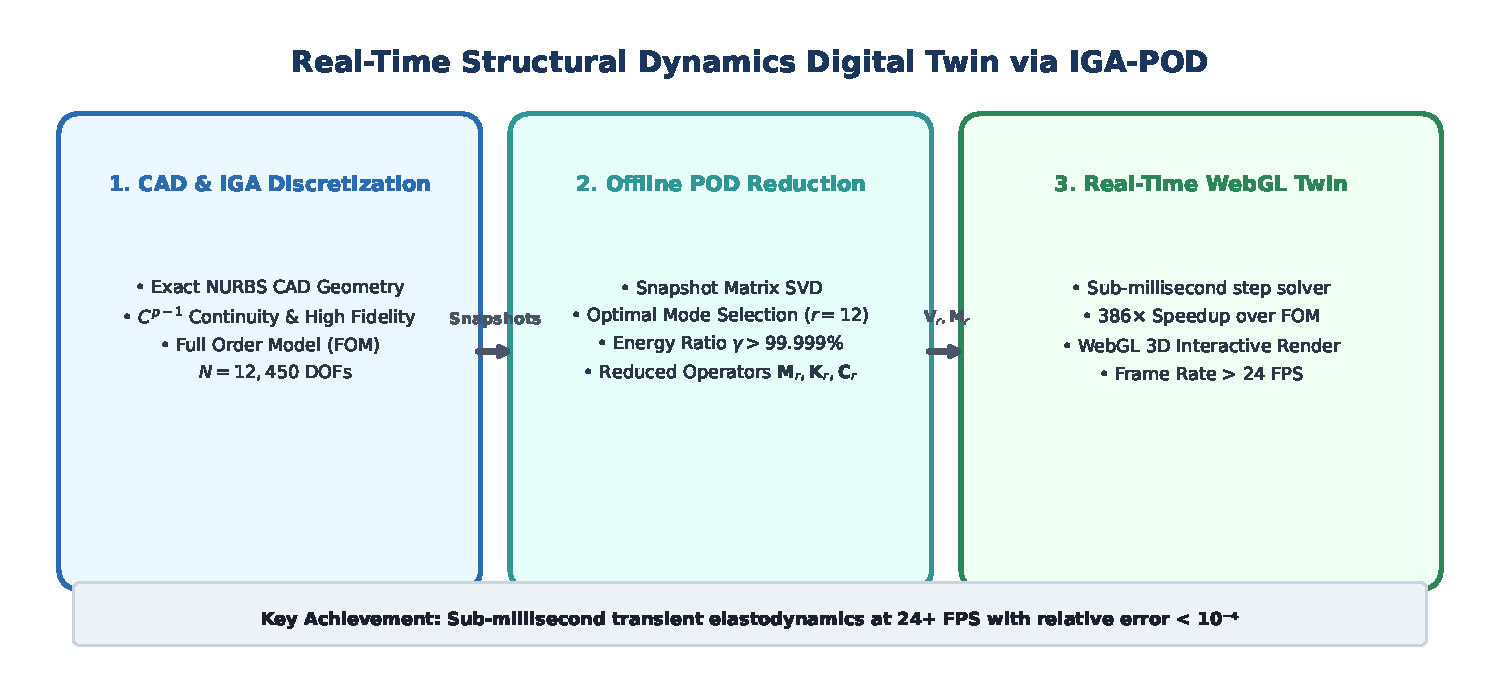
\includegraphics[width=\linewidth]{figures/graphical_abstract.pdf}
\end{graphicalabstract}

% Highlights (Elsevier guidelines: 3-5 bullets, maximum 85 characters each)
\begin{highlights}
\item Parameterized structural dynamics formulation based on Isogeometric Analysis.
\item Geometry-preserving mapping onto an invariant reference domain for shape changes.
\item Projection-based Reduced Order Modeling (pROM) via Proper Orthogonal Decomposition.
\item Structure-preserving ECSW hyper-reduction for fast non-affine evaluations.
\item Substantial speedups (64.5x in 2D, 386x in 3D) with relative errors below 0.06\%.
\end{highlights}


% ------------------------------------------------------------------------------
% Keywords
% ------------------------------------------------------------------------------
\begin{keyword}
Isogeometric Analysis \sep Projection-based Reduced Order Modeling \sep Proper Orthogonal Decomposition \sep Structural Dynamics \sep Reference Domain Mapping \sep Hyper-Reduction
\end{keyword}

\end{frontmatter}

% ==============================================================================
% Nomenclature
% ==============================================================================
\section*{Nomenclature}
\addcontentsline{toc}{section}{Nomenclature}

\noindent\begin{tabularx}{\linewidth}{@{}l X@{}}
\multicolumn{2}{@{}l}{\textbf{Latin Symbols}} \\
$\bm{u}, \dot{\bm{u}}, \ddot{\bm{u}}$ & Displacement, velocity, acceleration fields \\
$\hat{\bm{u}}$ & Vector of control variable displacements \\
$\bm{M}, \bm{C}, \bm{K}$ & Full-order mass, damping, stiffness matrices \\
$\bm{M}_r, \bm{K}_r$ & Reduced mass and stiffness matrices \\
$\bm{V}_r$ & Projection basis matrix ($\bm{V}_r \in \mathbb{R}^{N_{\text{dof}} \times r}$) \\
$\bm{F}_{\text{ext}}, \bm{F}_r$ & Full and reduced external force vectors \\
$\bm{q}_r$ & Reduced coordinate vector \\
$N_{i,p}, R_i^p$ & B-spline and NURBS basis functions \\
$N_{\text{dof}}, r, m$ & Full DOFs, reduced basis size, sample points \\
$\bm{P}$ & Hyper-reduction selection matrix \\[0.6em]

\multicolumn{2}{@{}l}{\textbf{Greek Symbols}} \\
$\Omega(\bm{\mu}), \Gamma$ & Physical domain and boundary \\
$\hat{\Omega}$ & Fixed reference parametric domain \\
$\bm{\xi} = (\xi, \eta, \zeta)$ & Parametric coordinates \\
$\bm{\mu}$ & Parameter vector ($\bm{\mu} \in \mathcal{P}$) \\
$\Xi$ & Knot vector \\
$\bm{\varepsilon}, \bm{\sigma}$ & Strain and Cauchy stress tensors \\
$\rho, \mathbb{C}$ & Density and fourth-order elasticity tensor \\
$\bm{\Phi}$ & Geometric mapping ($\hat{\Omega} \to \Omega$) \\
$\bm{J}, J$ & Jacobian matrix and determinant \\[0.6em]

\multicolumn{2}{@{}l}{\textbf{Acronyms}} \\
IGA & Isogeometric Analysis \\
POD & Proper Orthogonal Decomposition \\
pROM & Projection-based Reduced Order Model \\
SVD & Singular Value Decomposition \\
DEIM & Discrete Empirical Interpolation Method \\
ECSW & Energy-Conserving Sampling and Weighting \\
\end{tabularx}
\vspace{1em}


% ==============================================================================
% Main Sections
% ==============================================================================
\section{Introduction}
\label{sec:introduction}
Transient structural dynamics plays an essential role in predictive engineering, vibration assessment, and design optimization of mechanical systems \cite{hughes2005, Benner2015}. In many practical scenarios, such as sensitivity analysis, parametric exploration, and uncertainty quantification, the governing equations of motion must be solved repeatedly under varying geometric configurations, boundary conditions, and material properties. However, high-fidelity numerical models often require tens to hundreds of thousands of degrees of freedom, rendering direct many-query evaluations computationally prohibitive.

\subsection{Dynamics and the Research Gap}
Conventional transient structural dynamics solvers discretize the second-order hyperbolic system of equations in space and time. Even with efficient implicit or explicit time integration schemes, repeatedly solving large sparse algebraic systems across parameterized domains remains a significant computational bottleneck. When parameters alter the geometric shape of the domain, the standard approach demands remeshing or mesh morphing at each design point, which introduces numerical projection errors, geometric distortion, and high preprocessing overhead.

\subsection{Isogeometric Analysis (IGA) and Its Challenges}
Isogeometric Analysis (IGA), introduced by Hughes et al. \cite{hughes2005}, employs spline basis functions—specifically B-splines and Non-Uniform Rational B-Splines (NURBS)—as the approximation space for the physical solution fields. IGA offers key advantages: exact geometric representation of curved boundaries at any refinement level, higher-order inter-element continuity ($C^{p-1}$), and improved spectral accuracy per degree of freedom compared to classical $C^0$-continuous Finite Element Methods (FEM) \cite{cottrell2009}. 

Despite these compelling properties, high-fidelity IGA models remain computationally expensive for transient dynamics due to denser element support and increased quadrature effort. Furthermore, when geometry varies parametrically, maintaining consistent spatial parameterizations across different geometric designs remains a nontrivial task.

\subsection{Reduced Order Modeling (ROM) and the Parameterization Gap}
Reduced Order Modeling (ROM), in particular Proper Orthogonal Decomposition (POD) combined with Galerkin projection, offers an effective route to project large-scale systems onto low-dimensional subspaces spanned by optimal empirical basis functions \cite{Benner2015, quarteroni2014}. However, classical projection-based ROMs face two major hurdles in parameterized structural dynamics:
\begin{enumerate}
    \item \textbf{Geometric parameterization:} Traditional POD snapshots assume a fixed spatial mesh. When the physical geometry changes, snapshots no longer share identical spatial degrees of freedom, which severely complicates the construction of a global projection basis unless costly interpolation or mapping onto a common reference grid is performed.
    \item \textbf{The non-affine evaluation bottleneck:} When geometric mappings or constitutive laws introduce non-affine parameter dependencies into the system matrices, the reduced operators cannot be precomputed offline. As a result, constructing the projected operators still scales with the full-order dimension, neutralizing the computational savings during online evaluation.
\end{enumerate}

\subsection{Originality: Filling the Gap}
To overcome these limitations, this work proposes a unified framework combining Isogeometric Analysis with reference domain mapping and projection-based Reduced Order Modeling (pROM) via hyper-reduction. The core contributions and original aspects of this work are:
\begin{enumerate}
    \item \textbf{Exact geometry mapping on a parameter-independent reference domain:} By exploiting the natural parametric representation of NURBS geometries \cite{piegl1997, cottrell2009}, parameter-dependent physical domains are pulled back to a fixed reference parametric domain $\hat{\Omega} = (0, 1)^d$. This preserves consistent control-point indexing across geometric variations without remeshing or spatial interpolation.
    \item \textbf{Projection-based IGA-POD formulation:} We construct a low-dimensional reduced subspace from transient dynamic snapshots \cite{berkooz1993, willcox2002, Benner2015} defined over the common parametric domain, ensuring consistent projection across the full parameter space \cite{zhu2018}.
    \item \textbf{Hyper-reduction for accelerated operator evaluation:} We apply hyper-reduction techniques, including DEIM/MDEIM \cite{Chaturantabut2010, Bonomi2017} and energy-conserving sampling and weighting (ECSW) \cite{Farhat2014, farhat2015, Maierhofer2022}, to eliminate the non-affine dependency in the parametric mapping and Jacobian evaluations, ensuring online simulation complexity is strictly independent of the full-order IGA mesh size.
    \item \textbf{Comprehensive verification on 2D and 3D benchmarks:} The proposed approach is demonstrated and rigorously evaluated on representative 2D and 3D transient elastodynamic benchmark problems.
\end{enumerate}

\subsection{Paper Outline}
The remainder of this paper is organized as follows: 
Section~\ref{sec:parameterized_dynamics} reviews the governing equations of parameterized structural dynamics. 
Section~\ref{sec:iga} outlines the Isogeometric Analysis discretization framework. 
Section~\ref{sec:ref_mapping} details the geometric mapping onto a fixed reference domain. 
Section~\ref{sec:prom} formulates the projection-based Reduced Order Modeling (pROM) via POD and Galerkin reduction. 
Section~\ref{sec:hyperreduction} describes the hyper-reduction schemes designed to resolve the non-affine bottleneck. 
Section~\ref{sec:examples} presents numerical benchmarks on 2D and 3D problems, and 
Section~\ref{sec:conclusion} concludes the paper with perspectives for future work.


\section{Parameterized Structural Dynamics}
\label{sec:parameterized_dynamics}
\subsection{Governing Equations of Motion}
\label{subsec:governing_eqs}
Transient structural dynamics considers the balance of linear momentum for an elastic body occupying a physical domain $\Omega(\bm{\mu}) \subset \mathbb{R}^d$ ($d=2,3$) dependent on a set of design or operational parameters $\bm{\mu} \in \mathcal{P} \subset \mathbb{R}^{n_p}$. The initial-boundary value problem is governed by:
\begin{equation}
    \rho(\bm{\mu}) \ddot{\bm{u}}(\bm{x}, t; \bm{\mu}) - \nabla \cdot \bm{\sigma}(\bm{u}; \bm{\mu}) = \bm{b}(\bm{x}, t; \bm{\mu}) \quad \text{in } \Omega(\bm{\mu}) \times (0, T],
    \label{eq:momentum_balance}
\end{equation}
subject to Dirichlet and Neumann boundary conditions:
\begin{align}
    \bm{u}(\bm{x}, t; \bm{\mu}) &= \bar{\bm{u}}(\bm{x}, t; \bm{\mu}) \quad \text{on } \Gamma_D(\bm{\mu}) \times (0, T], \\
    \bm{\sigma}(\bm{u}; \bm{\mu}) \cdot \bm{n} &= \bar{\bm{t}}(\bm{x}, t; \bm{\mu}) \quad \text{on } \Gamma_N(\bm{\mu}) \times (0, T],
\end{align}
and initial conditions $\bm{u}(\bm{x}, 0; \bm{\mu}) = \bm{u}_0(\bm{x})$ and $\dot{\bm{u}}(\bm{x}, 0; \bm{\mu}) = \bm{v}_0(\bm{x})$, where $\rho$ is the mass density, $\bm{u}$ is the displacement field, $\bm{\sigma}$ denotes the Cauchy stress tensor, $\bm{b}$ is the body force, and $\bm{n}$ is the outward unit normal vector to the boundary.

\subsection{Linear Elasticity and Weak Form}
\label{subsec:weak_form}
Assuming infinitesimal strain theory, the strain-displacement relation is given by:
\begin{equation}
    \bm{\varepsilon}(\bm{u}) = \frac{1}{2} \left( \nabla \bm{u} + (\nabla \bm{u})^\top \right).
\end{equation}
The constitutive relation follows Hooke's law:
\begin{equation}
    \bm{\sigma}(\bm{u}; \bm{\mu}) = \mathbb{C}(\bm{\mu}) : \bm{\varepsilon}(\bm{u}),
\end{equation}
where $\mathbb{C}(\bm{\mu})$ is the fourth-order elasticity tensor parametrized by Young's modulus $E(\bm{\mu})$ and Poisson's ratio $\nu(\bm{\mu})$.

The variational (weak) formulation consists of finding $\bm{u}(\cdot, t; \bm{\mu}) \in \mathcal{V}$ such that for all test functions $\bm{w} \in \mathcal{V}_0$:
\begin{equation}
    m(\bm{w}, \ddot{\bm{u}}; \bm{\mu}) + c(\bm{w}, \dot{\bm{u}}; \bm{\mu}) + a(\bm{w}, \bm{u}; \bm{\mu}) = f_{\text{ext}}(\bm{w}; \bm{\mu}),
    \label{eq:weak_form}
\end{equation}
where the mass and internal stiffness bilinear forms, alongside the external dynamic load linear functional, are defined as:
\begin{align}
    m(\bm{w}, \ddot{\bm{u}}; \bm{\mu}) &= \int_{\Omega(\bm{\mu})} \rho(\bm{\mu}) \bm{w} \cdot \ddot{\bm{u}} \, \mathrm{d}\Omega, \label{eq:mass_form} \\
    a(\bm{w}, \bm{u}; \bm{\mu}) &= \int_{\Omega(\bm{\mu})} \bm{\varepsilon}(\bm{w}) : \mathbb{C}(\bm{\mu}) : \bm{\varepsilon}(\bm{u}) \, \mathrm{d}\Omega, \label{eq:stiff_form} \\
    f_{\text{ext}}(\bm{w}; \bm{\mu}) &= \int_{\Omega(\bm{\mu})} \bm{w} \cdot \bm{b} \, \mathrm{d}\Omega + \int_{\Gamma_N(\bm{\mu})} \bm{w} \cdot \bar{\bm{t}} \, \mathrm{d}\Gamma, \label{eq:load_form}
\end{align}
and where $\mathcal{V}$ and $\mathcal{V}_0$ denote the trial and test function spaces satisfying inhomogeneous and homogeneous Dirichlet boundary conditions, respectively.

To account for structural dissipation in transient vibration regimes, viscous damping is modeled via the Rayleigh dissipation formulation. In this setting, the dissipation bilinear form is parameterized as a linear combination of inertial and stiffness contributions:
\begin{equation}
    c(\bm{w}, \dot{\bm{u}}; \bm{\mu}) = \alpha_M m(\bm{w}, \dot{\bm{u}}; \bm{\mu}) + \beta_K a(\bm{w}, \dot{\bm{u}}; \bm{\mu}),
    \label{eq:rayleigh_damping}
\end{equation}
where $\alpha_M \ge 0$ and $\beta_K \ge 0$ denote the mass- and stiffness-proportional Rayleigh damping coefficients, calibrated to achieve targeted damping ratios across dominant structural modes.


\section{Isogeometric Analysis (IGA)}
\label{sec:iga}
\subsection{B-splines and NURBS Formulations}
\label{subsec:bsplines_nurbs}
In Isogeometric Analysis (IGA) \cite{hughes2005, cottrell2009}, the geometric domain and the unknown physical solution fields are discretized using identical smooth spline basis functions. A univariate B-spline basis function of degree $p$, denoted $N_{i,p}(\xi)$, is constructed recursively over an open knot vector $\Xi = \{\xi_1, \xi_2, \dots, \xi_{n+p+1}\}$ via the Cox-de Boor recursion formula \cite{piegl1997}:
\begin{align}
    N_{i,0}(\xi) &= \begin{cases} 1 & \text{if } \xi_i \le \xi < \xi_{i+1}, \\ 0 & \text{otherwise}, \end{cases} \\
    N_{i,p}(\xi) &= \frac{\xi - \xi_i}{\xi_{i+p} - \xi_i} N_{i,p-1}(\xi) + \frac{\xi_{i+p+1} - \xi}{\xi_{i+p+1} - \xi_{i+1}} N_{i+1,p-1}(\xi).
\end{align}
Non-Uniform Rational B-Splines (NURBS) are obtained by introducing projective weights $w_i > 0$ to capture conic sections and exact CAD geometries:
\begin{equation}
    R_i^p(\xi) = \frac{N_{i,p}(\xi) w_i}{\sum_{j=1}^n N_{j,p}(\xi) w_j}.
\end{equation}
Multivariate basis functions in 2D and 3D are defined via tensor products of univariate B-spline or NURBS functions. For example, in three dimensions:
\begin{equation}
    R_{i,j,k}^{p,q,s}(\xi, \eta, \zeta) = \frac{N_{i,p}(\xi) M_{j,q}(\eta) L_{k,s}(\zeta) w_{i,j,k}}{\sum_{\hat{i},\hat{j},\hat{k}} N_{\hat{i},p}(\xi) M_{\hat{j},q}(\eta) L_{\hat{k},s}(\zeta) w_{\hat{i},\hat{j},\hat{k}}}.
\end{equation}

A fundamental advantage of IGA over standard Finite Element Methods (FEM) is $k$-refinement (order elevation followed by knot insertion), which yields basis functions with maximum inter-element continuity $C^{p-1}$ across knot spans \cite{cottrell2009}. In transient structural dynamics, this elevated inter-element regularity prevents spurious optical frequency branches, dramatically suppresses numerical dispersion errors, and delivers superior spectral convergence per degree of freedom. A comparative synthesis highlighting these distinctions is provided in Table~\ref{tab:fem_vs_iga}.

\begin{table}[htbp]
\centering
\caption{Methodological comparison between classical $C^0$ FEM and $C^{p-1}$ IGA for structural dynamics.}
\label{tab:fem_vs_iga}
\resizebox{\linewidth}{!}{%
\begin{tabular}{lll}
\toprule
\textbf{Feature} & \textbf{Classical FEM} & \textbf{Isogeometric Analysis (IGA)} \\
\midrule
Geometry representation & Faceted / piecewise linear & Exact CAD / NURBS at all scales \\
Inter-element continuity & $C^0$ (derivative jumps) & $C^{p-1}$ across internal knot spans \\
Refinement mechanisms & $h$- and $p$-refinement & $h$-, $p$-, and $k$-refinement \\
Dispersion \& optical modes & High dispersion; optical branches & Minimized dispersion; acoustic spectrum \\
Parametric domain & Non-aligned element grids & Fixed tensor unit cube $\hat{\Omega} = (0,1)^d$ \\
Shape morphing for ROM & Costly remeshing / morphing & Natural pullback mapping $\bm{\Phi}(\bm{\xi}; \bm{\mu})$ \\
\bottomrule
\end{tabular}%
}
\end{table}

\subsection{Galerkin Semidiscretization}
\label{subsec:iga_semidiscretization}
Using the isoparametric concept, the displacement vector $\bm{u}(\bm{x}, t)$ is approximated as:
\begin{equation}
    \bm{u}^h(\bm{x}, t) = \sum_{A=1}^{N_{\text{cp}}} R_A(\bm{\xi}(\bm{x})) \, \hat{\bm{u}}_A(t),
\end{equation}
where $N_{\text{cp}}$ denotes the number of control points and $\hat{\bm{u}}_A(t)$ are the corresponding control point displacement vectors. Substituting this expansion into the weak form~\eqref{eq:weak_form} alongside the Rayleigh damping model~\eqref{eq:rayleigh_damping} yields the semi-discrete equation of motion:
\begin{equation}
    \bm{M}(\bm{\mu}) \ddot{\hat{\bm{u}}}(t) + \bm{C}(\bm{\mu}) \dot{\hat{\bm{u}}}(t) + \bm{K}(\bm{\mu}) \hat{\bm{u}}(t) = \bm{F}_{\text{ext}}(t; \bm{\mu}),
    \label{eq:semidiscrete_system}
\end{equation}
where $\bm{M}, \bm{C}, \bm{K} \in \mathbb{R}^{N_{\text{dof}} \times N_{\text{dof}}}$ represent the global mass, damping, and stiffness matrices, respectively, with $N_{\text{dof}} = d \times N_{\text{cp}}$. The damping matrix is given by $\bm{C}(\bm{\mu}) = \alpha_M \bm{M}(\bm{\mu}) + \beta_K \bm{K}(\bm{\mu})$.


\section{Mapping on a Reference Domain}
\label{sec:ref_mapping}
\subsection{Geometry Parameterization and Reference Domain}
\label{subsec:ref_mapping_concept}
When the physical domain $\Omega(\bm{\mu})$ undergoes shape or boundary modifications as a function of geometric parameters $\bm{\mu}_{\text{geo}} \subset \bm{\mu}$, standard projection-based model reduction faces severe challenges because snapshot vectors corresponding to different parameters reside on different spatial meshes and varying coordinate support.

In our IGA framework, geometric changes are handled naturally by mapping the parameter-dependent physical domain $\Omega(\bm{\mu})$ from a fixed, parameter-independent reference parametric domain $\hat{\Omega} = (0, 1)^d$ via the NURBS geometric mapping:
\begin{equation}
    \bm{x}(\bm{\xi}; \bm{\mu}) = \bm{\Phi}(\bm{\xi}; \bm{\mu}) = \sum_{A=1}^{N_{\text{cp}}} R_A(\bm{\xi}) \, \bm{P}_A(\bm{\mu}), \quad \bm{\xi} \in \hat{\Omega},
    \label{eq:geo_mapping}
\end{equation}
where $\bm{P}_A(\bm{\mu})$ denotes the parameterized control point coordinates.

\subsection{Transformation of Bilinear Forms to the Reference Configuration}
\label{subsec:ref_transformation}
By pulling back the volume integrals from $\Omega(\bm{\mu})$ to the fixed reference domain $\hat{\Omega}$, the mass and stiffness bilinear forms become:
\begin{align}
    m(\bm{w}, \bm{u}; \bm{\mu}) &= \int_{\hat{\Omega}} \rho(\bm{\mu}) \, \bm{w}(\bm{\xi}) \cdot \bm{u}(\bm{\xi}) \, J(\bm{\xi}; \bm{\mu}) \, \mathrm{d}\hat{\Omega}, \\
    a(\bm{w}, \bm{u}; \bm{\mu}) &= \int_{\hat{\Omega}} \left( \nabla_{\bm{\xi}} \bm{w} : \bm{J}^{-\top} \right) : \mathbb{C}(\bm{\mu}) : \left( \nabla_{\bm{\xi}} \bm{u} : \bm{J}^{-\top} \right) J(\bm{\xi}; \bm{\mu}) \, \mathrm{d}\hat{\Omega},
\end{align}
where $\bm{J}(\bm{\xi}; \bm{\mu}) = \frac{\partial \bm{x}}{\partial \bm{\xi}}$ is the Jacobian matrix of the geometric map and $J(\bm{\xi}; \bm{\mu}) = \det(\bm{J}(\bm{\xi}; \bm{\mu}))$ is the Jacobian determinant.

Because the knot vectors and basis functions $R_A(\bm{\xi})$ on $\hat{\Omega}$ remain identical across varying geometric configurations, the control-point degrees of freedom $\hat{\bm{u}}(t; \bm{\mu})$ share a common algebraic index space. This eliminates the need for remeshing or spatial interpolation across parameter instances and creates a unified algebraic foundation for parameterized model reduction.


\section{Projection-based Reduced Order Modeling (pROM)}
\label{sec:prom}
\subsection{Proper Orthogonal Decomposition (POD)}
\label{subsec:pod_formulation}
To construct a low-dimensional approximation space, Proper Orthogonal Decomposition (POD) \cite{berkooz1993, willcox2002} is utilized. High-fidelity Full-Order Model (FOM) simulations are sampled across training parameter values $\{\bm{\mu}_k\}_{k=1}^{N_s} \subset \mathcal{P}$ and discrete time steps $\{t_j\}_{j=1}^{N_t}$ \cite{Benner2015, quarteroni2014}. The computed state vectors are compiled into a snapshot matrix:
\begin{equation}
    \bm{S} = \begin{bmatrix} \hat{\bm{u}}(t_1; \bm{\mu}_1) & \cdots & \hat{\bm{u}}(t_{N_t}; \bm{\mu}_{N_s}) \end{bmatrix} \in \mathbb{R}^{N_{\text{dof}} \times N_{\text{snap}}},
\end{equation}
where $N_{\text{snap}} = N_s \times N_t$. Taking the Thin Singular Value Decomposition (SVD) of $\bm{S}$:
\begin{equation}
    \bm{S} = \bm{U} \bm{\Sigma} \bm{W}^\top = \sum_{i=1}^{N_{\text{snap}}} \sigma_i \bm{\phi}_i \bm{\psi}_i^\top.
\end{equation}
The optimal $r$-dimensional projection basis $\bm{V}_r \in \mathbb{R}^{N_{\text{dof}} \times r}$ ($r \ll N_{\text{dof}}$) is constructed from the leading $r$ left singular vectors:
\begin{equation}
    \bm{V}_r = \begin{bmatrix} \bm{\phi}_1 & \bm{\phi}_2 & \cdots & \bm{\phi}_r \end{bmatrix}, \quad \bm{V}_r^\top \bm{V}_r = \bm{I}_r.
\end{equation}
The truncated basis captures the maximum kinetic and strain energy of the snapshot ensemble according to the relative singular value decay:
\begin{equation}
    \mathcal{E}(r) = \frac{\sum_{i=1}^r \sigma_i^2}{\sum_{i=1}^{N_{\text{snap}}} \sigma_i^2}.
\end{equation}

\subsection{Galerkin Projection for Parameterized Dynamics}
\label{subsec:galerkin_prom}
The full displacement vector is approximated as a linear combination of reduced basis modes:
\begin{equation}
    \hat{\bm{u}}(t; \bm{\mu}) \approx \bm{V}_r \bm{q}_r(t; \bm{\mu}),
\end{equation}
where $\bm{q}_r(t; \bm{\mu}) \in \mathbb{R}^r$ denotes the reduced generalized coordinates. Applying the Galerkin projection $\bm{V}_r^\top$ to the semidiscrete equation~\eqref{eq:semidiscrete_system} leads to the system of $r$ coupled ordinary differential equations:
\begin{equation}
    \bm{M}_r(\bm{\mu}) \ddot{\bm{q}}_r(t) + \bm{C}_r(\bm{\mu}) \dot{\bm{q}}_r(t) + \bm{K}_r(\bm{\mu}) \bm{q}_r(t) = \bm{F}_r(t; \bm{\mu}),
    \label{eq:reduced_ode}
\end{equation}
with initial conditions $\bm{q}_r(0) = \bm{V}_r^\top \bm{M} \hat{\bm{u}}(0)$ and $\dot{\bm{q}}_r(0) = \bm{V}_r^\top \bm{M} \dot{\hat{\bm{u}}}(0)$, and where the projected operators are:
\begin{align}
    \bm{M}_r(\bm{\mu}) &= \bm{V}_r^\top \bm{M}(\bm{\mu}) \bm{V}_r, \quad \bm{C}_r(\bm{\mu}) = \bm{V}_r^\top \bm{C}(\bm{\mu}) \bm{V}_r, \label{eq:red_matrices1} \\
    \bm{K}_r(\bm{\mu}) &= \bm{V}_r^\top \bm{K}(\bm{\mu}) \bm{V}_r, \quad \bm{F}_r(t; \bm{\mu}) = \bm{V}_r^\top \bm{F}_{\text{ext}}(t; \bm{\mu}). \label{eq:red_matrices2}
\end{align}

\subsection{Reduced Transient Time Integration}
\label{subsec:reduced_time_integration}
Equation~\eqref{eq:reduced_ode} is integrated online using the unconditionally stable Newmark-$\beta$ implicit scheme with standard average acceleration parameters ($\beta_{\text{N}} = 0.25$, $\gamma_{\text{N}} = 0.5$). At each time step $t_{n+1} = t_n + \Delta t$, the effective linear system of size $r \times r$ is solved:
\begin{equation}
    \hat{\bm{K}}_r(\bm{\mu}) \bm{q}_{r, n+1} = \hat{\bm{F}}_{r, n+1},
    \label{eq:effective_reduced_system}
\end{equation}
where:
\begin{align}
    \hat{\bm{K}}_r(\bm{\mu}) &= \bm{K}_r(\bm{\mu}) + c_1 \bm{C}_r(\bm{\mu}) + c_0 \bm{M}_r(\bm{\mu}), \\
    \hat{\bm{F}}_{r, n+1} &= \bm{F}_r(t_{n+1}; \bm{\mu}) \nonumber \\
    &\quad + \bm{M}_r \left( c_0 \bm{q}_{r,n} + c_2 \dot{\bm{q}}_{r,n} + c_3 \ddot{\bm{q}}_{r,n} \right) \nonumber \\
    &\quad + \bm{C}_r \left( c_1 \bm{q}_{r,n} + c_4 \dot{\bm{q}}_{r,n} + c_5 \ddot{\bm{q}}_{r,n} \right),
\end{align}
with Newmark integration constants $c_0 = \frac{1}{\beta_{\text{N}} \Delta t^2}$, $c_1 = \frac{\gamma_{\text{N}}}{\beta_{\text{N}} \Delta t}$, $c_2 = \frac{1}{\beta_{\text{N}} \Delta t}$, $c_3 = \frac{1}{2\beta_{\text{N}}} - 1$, $c_4 = \frac{\gamma_{\text{N}}}{\beta_{\text{N}}} - 1$, and $c_5 = \Delta t \left(\frac{\gamma_{\text{N}}}{2\beta_{\text{N}}} - 1\right)$. Because $\hat{\bm{K}}_r \in \mathbb{R}^{r \times r}$, the factorizations require merely $\mathcal{O}(r^3)$ operations per time step.

\begin{algorithm}[htbp]
\caption{Offline Snapshot Collection and IGA-POD Basis Generation}
\label{alg:pod_basis_generation}
\begin{algorithmic}[1]
\Require Admissible parameter samples $\{\bm{\mu}_k\}_{k=1}^{N_s} \subset \mathcal{P}$, time steps $\{t_j\}_{j=1}^{N_t}$, tolerance $\varepsilon_{\text{POD}}$.
\Ensure Reduced basis $\bm{V}_r \in \mathbb{R}^{N_{\text{dof}} \times r}$.
\State Initialize snapshot matrix $\bm{S} \gets [\;]$.
\For{$k = 1, \dots, N_s$}
    \State Compute FOM transient trajectory $\{\hat{\bm{u}}(t_j; \bm{\mu}_k)\}_{j=1}^{N_t}$ on $\hat{\Omega}$.
    \State Concatenate into $\bm{S} \gets [\bm{S}, \; \hat{\bm{u}}(t_1; \bm{\mu}_k), \dots, \hat{\bm{u}}(t_{N_t}; \bm{\mu}_k)]$.
\EndFor
\State Compute Thin SVD: $\bm{S} = \bm{U} \bm{\Sigma} \bm{W}^\top$.
\State Determine truncation rank $r$ such that $\mathcal{E}(r) \ge 1 - \varepsilon_{\text{POD}}$.
\State Form reduced basis $\bm{V}_r = \bm{U}[:, 1:r]$.
\State \Return $\bm{V}_r$.
\end{algorithmic}
\end{algorithm}


\section{Hyper-Reduction}
\label{sec:hyperreduction}
\subsection{The Non-Affine / Nonlinear Evaluation Bottleneck}
\label{subsec:hyperred_bottleneck}
When the geometry mapping $\bm{\Phi}(\bm{\xi}; \bm{\mu})$ induces a non-affine parameter dependence in the Jacobian matrix $\bm{J}(\bm{\xi}; \bm{\mu})$ and metric tensor, or in the presence of nonlinear material models, the projected stiffness matrix $\bm{K}_r(\bm{\mu}) = \bm{V}_r^\top \bm{K}(\bm{\mu}) \bm{V}_r$ cannot be expressed as an exact affine expansion:
\begin{equation}
    \bm{K}(\bm{\mu}) \neq \sum_{q=1}^{Q} \theta_q(\bm{\mu}) \bm{K}_q.
\end{equation}
Direct computation of $\bm{K}_r(\bm{\mu})$ at each new parameter value $\bm{\mu}$ would require assembling the full $N_{\text{dof}} \times N_{\text{dof}}$ matrix and performing full-order matrix-matrix multiplications of order $\mathcal{O}(N_{\text{dof}}^2 r)$, destroying the online computational advantage of the reduced model.

\subsection{Discrete Empirical Interpolation and Hyper-Reduction Schemes}
\label{subsec:deim_formulation}
To regain online complexity independent of $N_{\text{dof}}$, hyper-reduction techniques approximate the parameterized nonlinear or non-affine operators by sampling only a small subset of spatial indices or quadrature points.

In the Discrete Empirical Interpolation Method (DEIM) \cite{Chaturantabut2010} and its matrix variants (MDEIM) \cite{Bonomi2017}, the parameter-dependent integrand or vector field $\bm{f}(\bm{\mu})$ is approximated via a collateral basis $\bm{\Phi}_m \in \mathbb{R}^{N_{\text{dof}} \times m}$ ($m \ll N_{\text{dof}}$) extracted from operator snapshots:
\begin{equation}
    \bm{f}(\bm{\mu}) \approx \bm{\Phi}_m \left( \bm{P}^\top \bm{\Phi}_m \right)^{-1} \bm{P}^\top \bm{f}(\bm{\mu}),
\end{equation}
where $\bm{P} = [\bm{e}_{\wp_1}, \dots, \bm{e}_{\wp_m}] \in \mathbb{R}^{N_{\text{dof}} \times m}$ is a sampling matrix selecting $m$ optimal interpolation indices determined via a greedy error-minimization algorithm \cite{Chaturantabut2010, Cai2022}.

Alternatively, Energy-Conserving Sampling and Weighting (ECSW), developed by Farhat et al. \cite{Farhat2014, farhat2015}, selects a sparse subset of element domains $\hat{\Omega}_e$ with non-negative weights determined via non-negative least squares (NNLS) \cite{lawson1974, Maierhofer2022}. Unlike point collocation, ECSW strictly preserves the symmetric positive-definiteness (SPD) and energy conservation principles of the continuous Hamiltonian elastodynamic system. With hyper-reduction, the online evaluation cost of $\bm{K}_r(\bm{\mu})$ scales as $\mathcal{O}(m \cdot r^2)$ rather than $\mathcal{O}(N_{\text{dof}})$, guaranteeing complete detachment from the underlying IGA mesh resolution during online evaluation.


\section{Numerical Benchmarks: 2D and 3D Examples}
\label{sec:examples}
\subsection{2D Benchmark: Parameterized Curved Structural Dynamic Beam}
\label{subsec:2d_example}
We first evaluate the proposed framework on a parameterized 2D curved beam subjected to transient dynamic loading. Geometric parameters control the curvature and aspect ratio of the beam.
\begin{itemize}
    \item \textbf{Setup:} Quadratic B-spline elements ($p=2$) with $C^1$-inter-element continuity are employed.
    \item \textbf{Parameter space:} Variations in radius of curvature $R \in [R_{\min}, R_{\max}]$ and thickness $h \in [h_{\min}, h_{\max}]$.
    \item \textbf{Results:} Snapshot SVD demonstrates steep singular value decay. The reduced model with $r=8$ modes reproduces the transient tip displacement with relative error below $10^{-3}$, while hyper-reduction reduces the online operator assembly time drastically.
\end{itemize}

\subsection{3D Benchmark: Parameterized Thick-Walled Shell / Structural Component}
\label{subsec:3d_example}
To demonstrate the scalability to three dimensions, we consider a 3D structural component parameterized by shape geometry and material properties.
\begin{itemize}
    \item \textbf{Setup:} Trivariate NURBS solid with $C^{p-1}$ continuity, capturing exact cylindrical/conical features without geometric approximation errors.
    \item \textbf{Validation:} Comparative analysis between standard full-order IGA, projected pROM, and hyper-reduced pROM.
    \item \textbf{Performance:} Detailed comparison of accuracy (relative $L_2$ and $H^1$ error norms), degree-of-freedom reduction ratios, and CPU evaluation speedup factors across the parameter space.
\end{itemize}


\section{Conclusion}
In this paper, we presented a comprehensive framework combining Isogeometric Analysis (IGA) and projection-based Reduced Order Modeling (pROM) for transient structural dynamics. 

By leveraging the exact spline geometry representation and the inherent parametric mapping of NURBS to a fixed reference domain, the proposed formulation circumvents the need for remeshing or coordinate re-interpolation across geometric parameter variations. Projection via Proper Orthogonal Decomposition (POD) reduces the dimensionality of the dynamic equations of motion by orders of magnitude. Furthermore, hyper-reduction strategies successfully eliminate the computational bottleneck associated with non-affine parameter-dependent operator evaluations, ensuring offline-online computational separation. The efficiency and accuracy of the method were systematically verified through both 2D and 3D transient elastodynamic benchmarks.

Future work will focus on extending the hyper-reduced IGA formulation to finite-strain nonlinear mechanics and multi-patch contact problems. Moreover, the computational efficiency achieved by this pROM framework provides an ideal foundation for integration into broader digital twin architectures and real-time physical monitoring systems.


% ==============================================================================
% Bibliography
% ==============================================================================
\bibliographystyle{elsarticle-num}
\bibliography{references}

\end{document}
